\begin{figure}[ht]
    \centering
    \begin{subfigure}[t]{0.49\linewidth}
        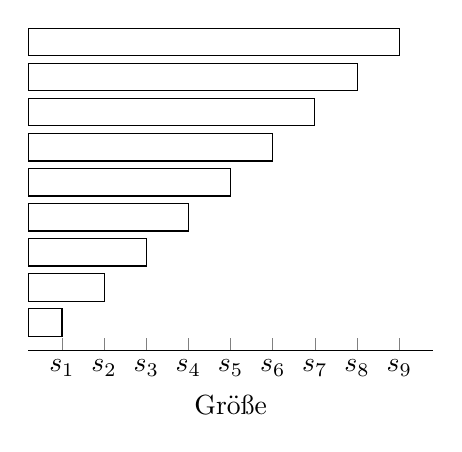
\begin{tikzpicture}
        \begin{axis}[
            xbar,
            xlabel={Größe},
            yticklabels=\empty,
            xtick={1, ..., 9},
            xticklabels={$s_1$, $s_2$, $s_3$, $s_4$, $s_5$, $s_6$, $s_7$, $s_8$, $s_9$},
            scale=0.75,
            axis y line=none,
            axis x line*=bottom,
        ]
            \addplot+ [fill=white, draw=black] coordinates  {(9, 9) (8, 8) (7, 7) (6, 6) (5, 5) (4, 4) (3, 3) (2, 2) (1, 1)};
        \end{axis}
        \end{tikzpicture}
        
        \subcaption{Größe der Eingangsmengen, dargestellt als Balkendiagramm.}
    \end{subfigure}
    \begin{subfigure}[t]{0.49\linewidth}
        \begin{tikzpicture}
        \begin{axis}[
            xlabel={Größe},
            ylabel={Zeit},
            yticklabels=\empty,
            xtick={0, ..., 8},
            xticklabels={$s_1$, $s_2$, $s_3$, $s_4$, $s_5$, $s_6$, $s_7$, $s_8$, $s_9$},
            scale=0.75,
            smooth,
            grid=major,
        ]
            \addplot [] table {data/example};
        \end{axis}
        \end{tikzpicture}

        \subcaption{$f(s)$}
    \end{subfigure}
    \caption{Beispielhafter Funktionsgraph der praktischen Effizienz eines hypothetischen Algorithmus mit Illustration der Eingabemengengrößen.}
    \label{fig:function-determination-example}
\end{figure}